\chapter{Casos de uso\label{cap:casos-de-uso}}
    Neste capítulo serão apresentados alguns sites e sistemas que firezam uso do \emph{Framework Lothus\{PHP\}}, demostrando a diversidade de projetos capazes de recebê-lo como ferramenta principal para o desenvolvimento.

    \section{Site institucional\label{sec:site-institucional}}

        Projeto que apresenta o uso do \emph{Framework} para desenvolvimento de um site institucional, que utiliza administração para controle de conteúdo.

        \begin{figure}[!htb]
            \centering
            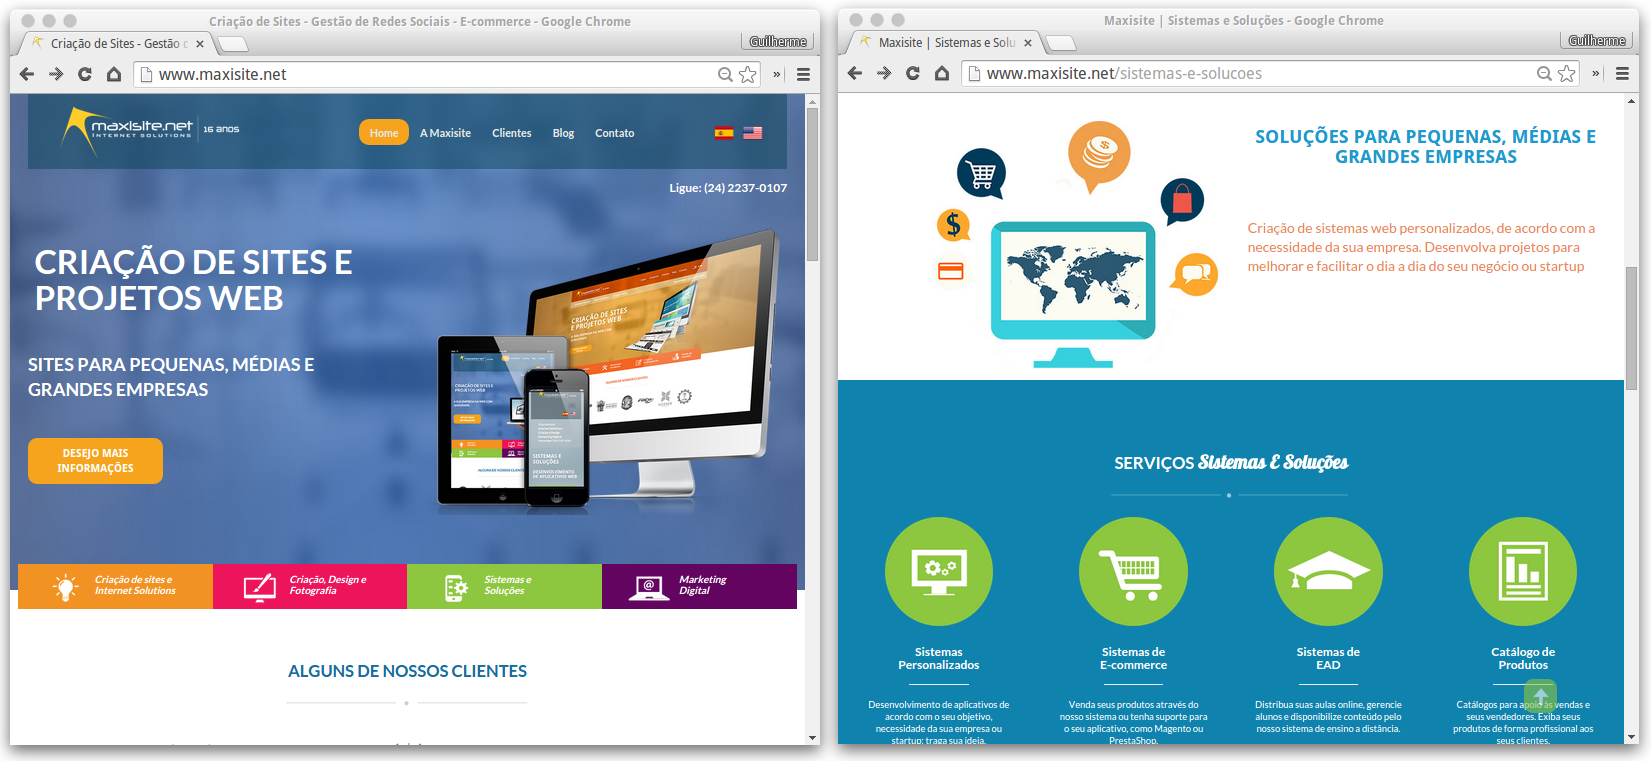
\includegraphics[scale=0.28]{maxisite.jpg}
            \caption{\small Exemplo de site institucional}
            \label{cap:sass}
        \end{figure}


    \section{Sistema de gestão\label{sec:sistema}}

        Este projeto demonstra o uso do \emph{Framework} para desenvolvimento de um sistema de gestão esportiva, fazendo uso de autenticação de usuários e divisão de grupos de permissão para área restrita.

        \begin{figure}[!htb]
            \centering
            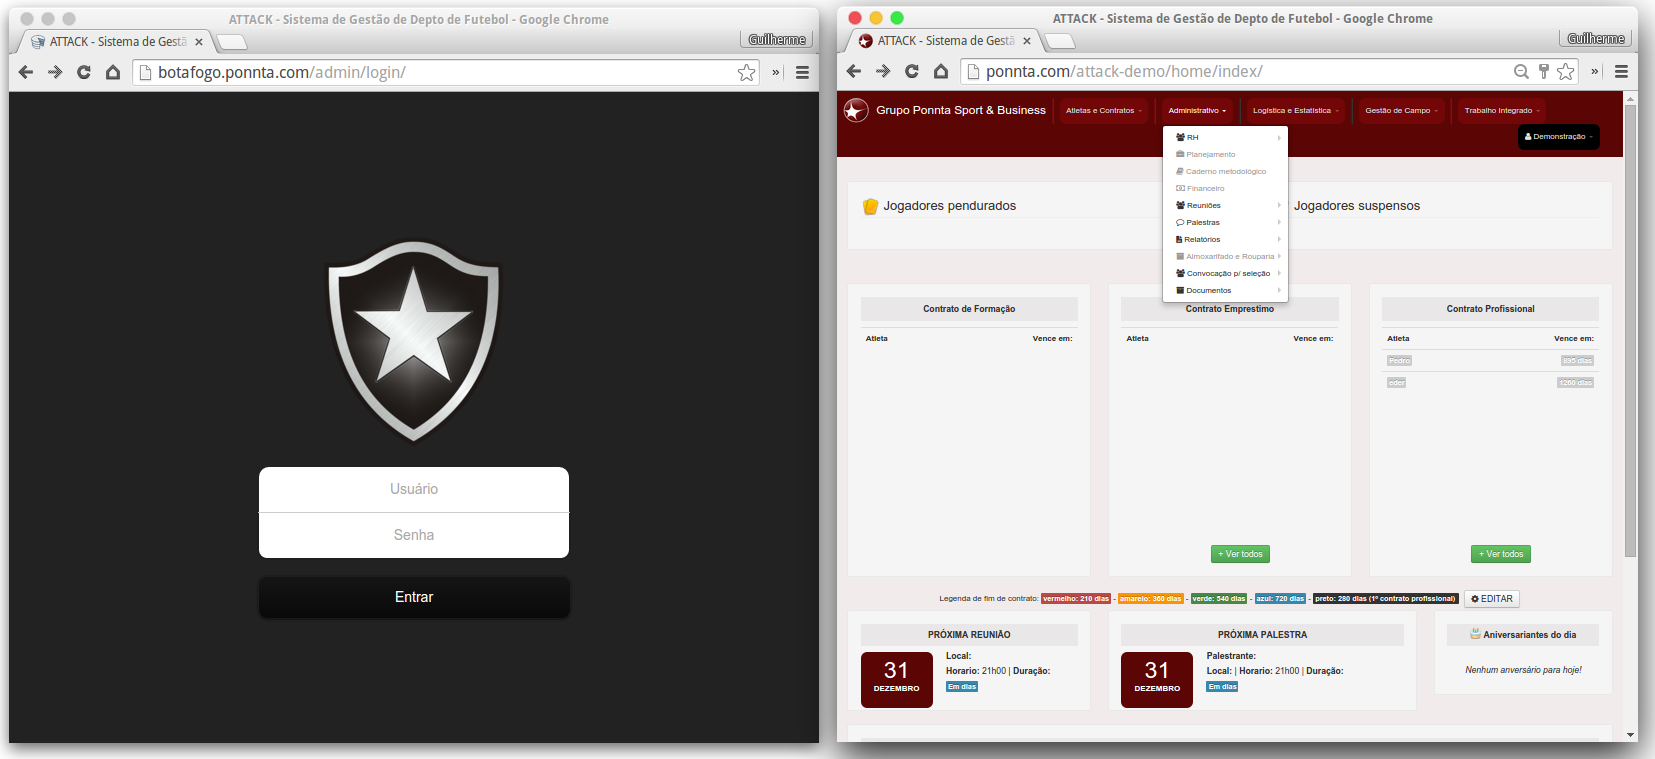
\includegraphics[scale=0.28]{attack.jpg}
            \caption{\small Exemplo de sistema de usuários}
            \label{cap:sass}
        \end{figure}


    \section{Portal de notícias\label{sec:portal}}

        Portal de notícias esportivas desenvolvido com o \emph{Framework Lothus\{PHP\}} e que faz uso de área administrativa para controle de conteúdo.

        \begin{figure}[!htb]
            \centering
            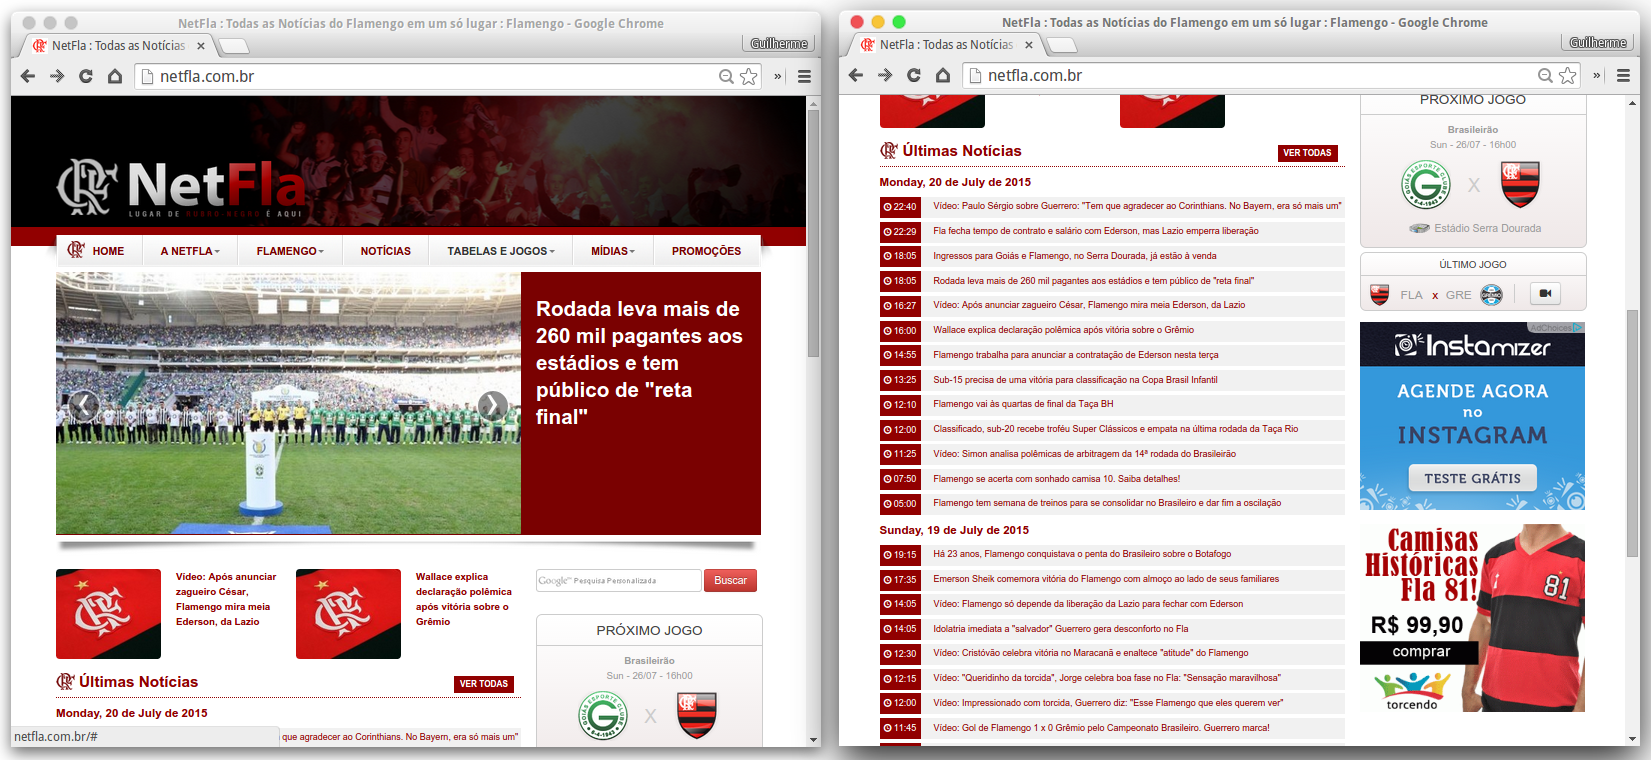
\includegraphics[scale=0.28]{netfla.jpg}
            \caption{\small Exemplo portal de notícias}
            \label{cap:sass}
        \end{figure}

        \emph{}

        \emph{}


    \section{E-commerce\label{sec:e-commerce}}

        Projeto de e-commerce utilizando o \emph{Framework} com pacotes para integração com pagamentos online e área restrita para controle de conteúdo e de vendas.

        \begin{figure}[!htb]
            \centering
            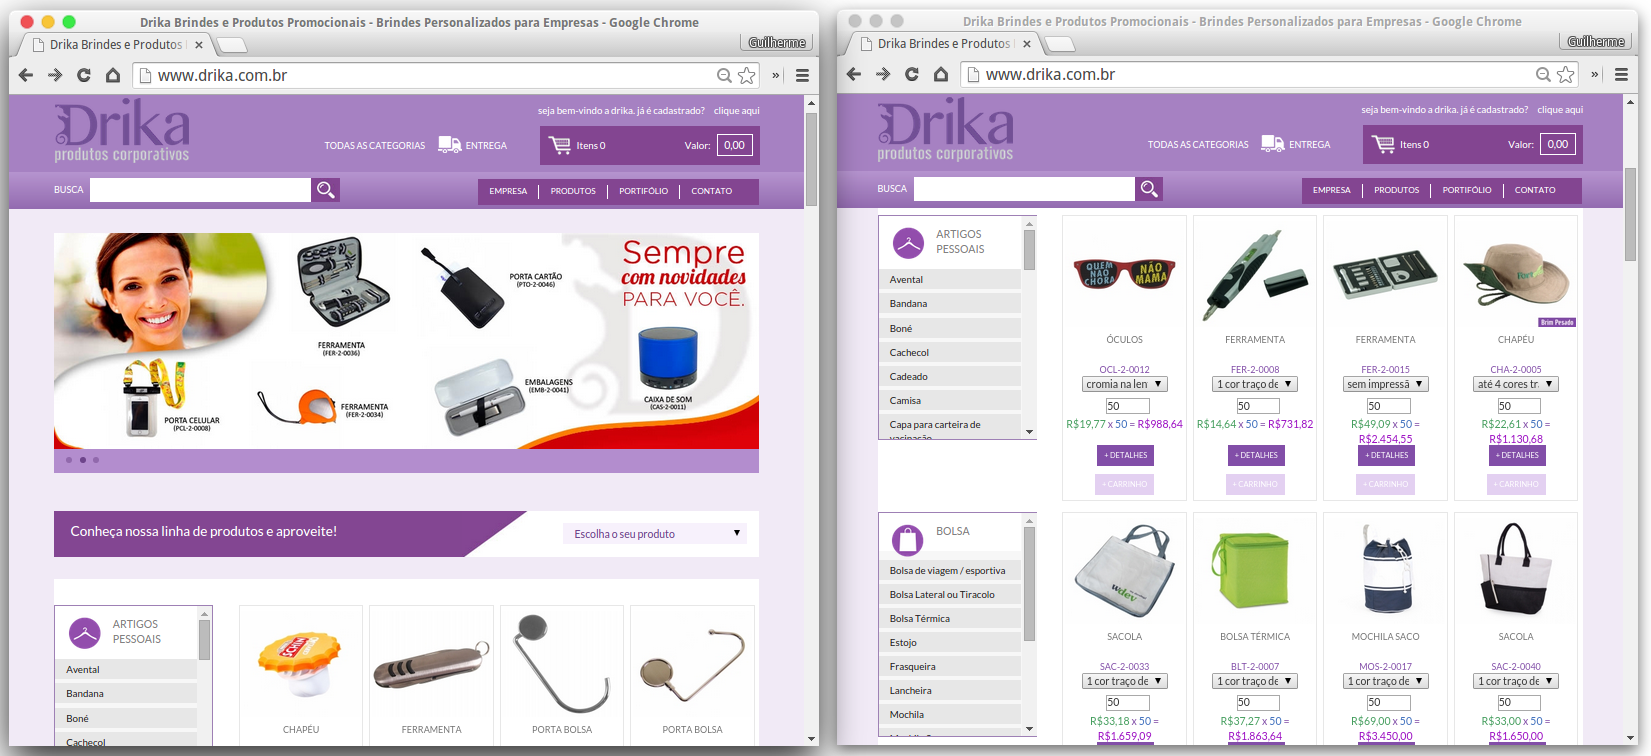
\includegraphics[scale=0.28]{drika.jpg}
            \caption{\small Exemplo de e-commerce}
            \label{cap:sass}
        \end{figure}